\chapter{Introduction} %\label{ch:intro}

In Synthetic Aperture Radar (SAR) imaging, radar antennas are mounted on an airborne or spaceborne platform. The scene to be imaged is illuminated by electromagnetic waves transmitted from an antenna. The goal is to extract information of the scene from the measurements taken of the scattered waves.

\section{Zero Point Energy and Dynamical Casimir Effect}
\section{Cavity QED and Superconducting circuits}
\section{DCE in Superconducting Circuits}
\section{Periodic Potentials and Bloch Theorem for Electrons}
 %\cite{Garza:2011fk}

\begin{equation} %\label{eq:einstein}
	e = mc^{2}
\end{equation}


\begin{comment}
\begin{figure}
  \centering
  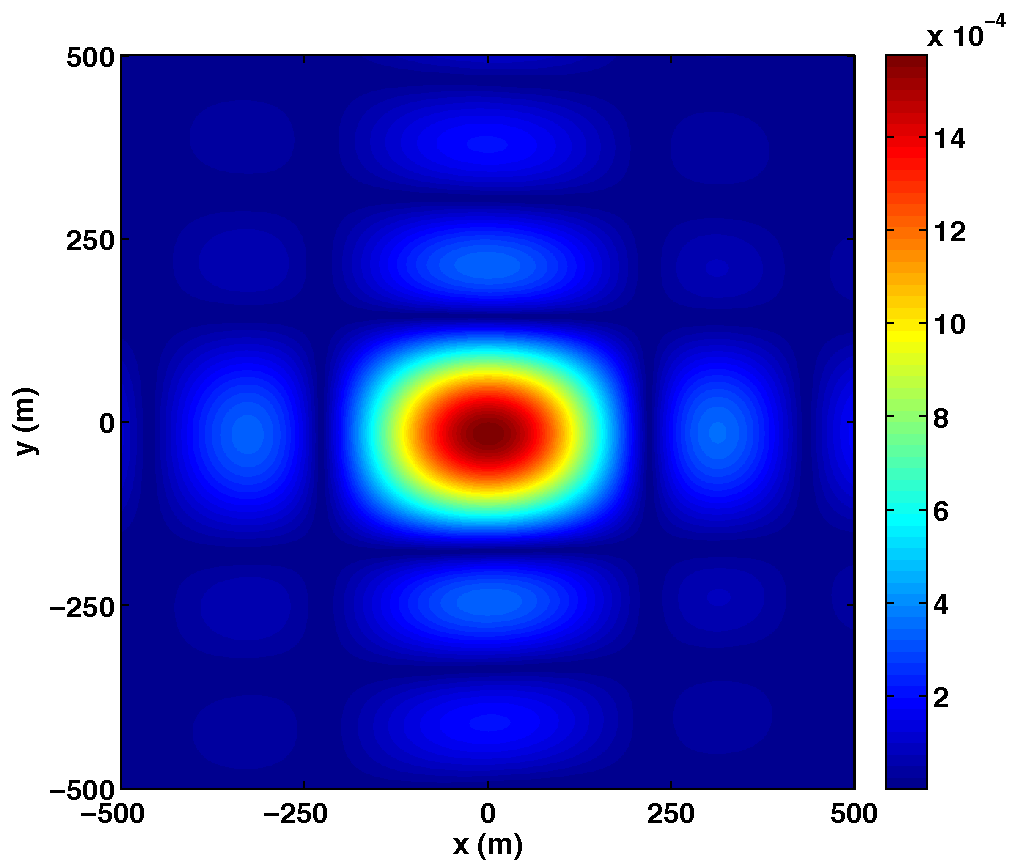
\includegraphics[scale=0.5]{figures/beamfootprint}
  \caption[Colorful Picture]{This is a colorful picture.}%
  \label{fig:flyover}
\end{figure}
\end{comment}


\begin{comment}
\begin{table}[p]
  \centering
\begin{tabular}{llr}
\toprule
\multicolumn{2}{c}{Item} \\
\cmidrule(r){1-2}
Animal    & Description & Price (\$) \\
\midrule
Gnat      & per gram    & 13.65      \\
          & each        & 0.01       \\
Gnu       & stuffed     & 92.50      \\
Emu       & stuffed     & 33.33      \\
Armadillo & frozen      & 8.99       \\
\bottomrule
\end{tabular}
  \caption[Table Example]{This table shows some data}%
  \label{tab:myfirsttable}
\end{table}
\end{comment}
